\documentclass[degree=doctor,bibtype=numeric]{tongjithesis}
\usepackage{tongjiutils}

%参考文献更新使用biblatex包, 使用gb7714-2015标准, 具体参数设置可在cls文件中搜索biblatex进行了解
%加入bib文件(老版本文件依然能够使用)
\usepackage{tongjiutils}

%参考文献更新使用biblatex包, 使用gb7714-2015标准, 具体参数设置可在cls文件中搜索biblatex进行了解
%加入bib文件(老版本文件依然能够使用)
\addbibresource{ref/refs.bib}   %


\begin{document}

% 定义所有的eps文件在 figures 子目录下
\graphicspath{{figures/}}


%%% 封面部分
\frontmatter
\tongjisetup{
  %******************************
  % 注意:
  %   1. 配置里面不要出现空行
  %   2. 不需要的配置信息可以删除
  %******************************
  %
  %=====
  % 秘级
  %=====
  secretlevel={保密},
  secretyear={2},
  % doctor={0}
  %
  %=========
  % 中文信息
  %=========
  % 题目过长可以换行(推荐手动加入换行符,这样就可以控制换行的地方啦)。
  ctitle={蛋白质复合物筛选模型研究},
  cheadingtitle={蛋白质复合物筛选模型研究},    %用于页眉的标题,不要换行
  %cauthor={高盼},
  %studentnumber={1830801},
  cmajorfirst={工学},
  cmajorsecond={计算机科学与技术},
  cdepartment={电子与信息工程学院},
  %csupervisor={关佶红 教授},
  % 如果没有副指导老师或者校外指导老师,把{}中内容留空即可,或者直接注释掉。
  % cassosupervisor={裴刚 教授~(校外)}, % 副指导老师
  % 日期自动使用当前时间,若需手动指定,按如下方式修改:
  % cdate={\zhdigits{2018}年\zhnumber{11}月},
  % 没有基金的话就注释掉吧。
  cfunds={(国家自然基金项目(某项目)资助},
  %
  %=========
  % 英文信息
  %=========
  etitle={Study on protein complex screening model},
  %eauthor={Pan Gao},
  emajorfirst={Engineering},
  emajorsecond={Computer Science and Technology},
  edepartment={School of Electronic and Information Engineering},
  % 日期自动使用当前时间,若需手动指定,按如下方式修改:
  % edate={November,\ 2018},
  % efunds={(Supported by the Natural Science Foundation of China(No.61772367,U1936205))},    
  %esupervisor={Prof. JiHong Guan}
  % eassosupervisor={Prof. Gang Pei (XiaoWai)}
  % }
}
% 定义中英文摘要和关键字
\begin{cabstract}
  蛋白质复合物是蛋白质相互结合完成某一项生物功能的集合。生物学上蛋白质复合物的识别与研究对细胞组成分析、药物预测等至关重要。生物实验的方法可以识别蛋白质复合物,但其成本较高、周期较长,无法满足大规模数据时代的研究需求。
  现有的蛋白质复合物预测算法主要是基于计算的算法,将蛋白质之间广泛的相互作用抽象成图,蛋白质复合物抽象为图中的局部结构,此时蛋白质复合物预测问题转换为局部子图发现问题。复合物预测算法可以从互作网络中挖掘出大量的局部子图样本,但是由于预测算法本身的局限性,预测结果中会存在部分不符合复合物形成规律的样本。基于计算的复合物预测算法不具有对其预测结果的评价能力,无法识别并剔除这部分样本。

  为了识别和剔除这部分对预测结果具有干扰性的样本,本文提出了蛋白质复合物筛选模型,构建了融合结点特征和邻边特征的蛋白质相互作用网络,并进一步构造了复合物特征子图样本集。本文提出了多种复合物筛选模型并针对每个模型进行了模型训练以及复合物筛选验证,复合物筛选模型包括基于图卷积的模型、基于邻边卷积的模型和基于点边消息传递网络的模型。

  本文的研究工作及贡献:

  1)融合结点特征和邻边特征的蛋白质相互作用网络(简称特征互作网络)。基于蛋白质互作数据构建了蛋白质相互作用网络,基于图自编码器、深度随机游走等网络嵌入方法为网络添加了结点特征,基于生物学上的多种相似性特征提取方法为网络添加了邻边特征,最终构建出特征互作网络。

  构造了多种类别的蛋白质复合物特征子图样本集。原始蛋白质复合物数据集以蛋白质集合的形式存在,无法满足样本后筛选工作的要求。本文基于特征子图提取方法,在特征互作网络中构建对应蛋白质复合物数据集的特征子图样本集,包括基于邻居相似性融合多个标准集构建的正样本数据集;基于COACH算法构建的中间样本数据集;基于改进的随机算法构建的负样本数据集;基于核心附属结构的复合物预测算法构建的待筛选数据集。

  2)基于图卷积神经网络的复合物筛选模型。从拓扑数据出发,本文提出了基于图卷积神经网络的复合物筛选模型。该模型基于图自编码器和深度随机游走嵌入得到蛋白质全局特征,并依据蛋白质复合物子图的拓扑结构,基于图神经网络对蛋白质全局特征进行深度融合。本文将该模型与无全局特征的模型、基于拓扑统计特征的模型进行了对比与分析,结果表明了融合全局特征的图卷积神经网络方法的有效性。
  
  3)基于邻边卷积的复合物筛选模型。从生物数据出发,针对蛋白质复合物生物数据抽象程度较低的问题,本文提出了基于邻边卷积的复合物筛选模型。该模型在蛋白质互作网络中嵌入了表达蛋白质功能关联的多种相似性数据,作为互作网络邻边特征,并基于邻边卷积的方法将子图拓扑和邻边特征进行融合。实验对比了有无邻边特征情况下的邻边卷积模型,结果显示了带邻边特征的邻边卷积模型的有效性。

  4)基于点边消息传递网络的复合物筛选模型。从特征融合角度出发,本文提出了基于点边消息传递网络的复合物筛选模型。该模型保留了表示全局拓扑特性的结点特征和表示生物功能特性的邻边特征,采用消息传递的更新方法在蛋白质复合物局部拓扑结构中同时更新结点特征和邻边特征,实现了全局拓扑特征与生物功能特征的动态更新和深度融合。结果表明基于点边消息传递网络地复合物筛选模型能更好地挖掘蛋白质复合物的形成规律,在多个实验中其评价指标的提升达到了最优。

\end{cabstract}

\ckeywords{蛋白质复合物预测;图神经网络;蛋白质相互作用网络;子图分类;图嵌入}

\begin{eabstract}
  A protein complex is a collection of proteins that bind to each other to accomplish a biological function. The identification and research of protein complexes in biology are very important for cell composition analysis, drug prediction and so on. The method of biological experiment can identify protein complex, but its cost is high and the cycle is long, which can not meet the research demand of large-scale data age.
  The existing protein complex prediction algorithm is mainly based on the calculation algorithm, abstracting the wide interaction between proteins into a diagram, protein complex abstraction into the local structure of the diagram, at which time the protein complex prediction problem is transformed into a local sub-graph to find the problem. The composite prediction algorithm can extract a large number of local subgraph samples from the mutual network, but due to the limitations of the prediction algorithm itself, there will be some samples in the prediction results that do not conform to the formation law of the compound. The calculation-based compound prediction algorithm does not have the ability to evaluate its prediction results, and cannot identify and reject this part of the sample.

  In order to identify and reject the samples which are disturbing to the prediction results, this paper presents a protein complex screening model, constructs a protein interaction network that combines node features and adjacent features, and further constructs a sample set of composite feature sub-maps. In this paper, a variety of composite filtering models are proposed and model training and composite filtering validation are carried out for each model, including models based on tortogram remnants, models based on adjacent curly volume, and models based on point edge messaging networks.

  The research work and contribution of this paper:

  1) A network of protein interactions (referred to as a network of features) that combines node features with adjacent features. Based on the protein interoperability data, the protein interaction network is constructed, the node characteristics are added to the network based on the network embedding methods such as graph self-encoder and deep random walk, and the adjacent features are added to the network based on various similarity characteristic extraction methods in biology, and the characteristic interoperability network is finally constructed.

  A sample set of sub-maps of protein complex features in various categories is constructed. The original protein complex dataset exists in the form of a protein collection and cannot meet the requirements of post-sample screening. Based on the feature sub-graph extraction method, this paper constructs the characteristic sub-map sample set of the corresponding protein complex data set in the feature interoperability network, including the positive sample data set built on the basis of multiple standard sets of neighbor similarity fusion, the intermediate sample data set based on THECH algorithm, the negative sample data set based on the improved random algorithm, and the pending filtering data set based on the composite prediction algorithm of the core satellite structure.


  2) A composite screening model based on a refride neural network. Based on the topological data, this paper presents a composite screening model based on the refride neural network. The model obtains the global characteristics of proteins based on graph self-encoder and deep random walk embedding, and based on the topology of protein complex subpic, the global characteristics of proteins are deeply fused based on the graph neural network. In this paper, the model is compared and analyzed with the model without global characteristics and based on topological statistical features, and the results show the effectiveness of the topographical neural network method of fusing global features.

  3) A composite filtering model based on neighboring coils. Based on the biological data, in view of the low abstraction of the biological data of protein complexes, this paper puts forward a composite screening model based on the neighboring reftric. The model embeds a variety of similarity data expressing protein function association in the protein interoperability network, as a mutual network neighbor feature, and fuses the subgraph topology and neighbor feature based on the method of neighbor converse. The experiment compares the neighborhood remnoms model with or without neighbor features, and the results show the validity of the neighboring reuter model with neighbor features.

  4)A composite filtering model based on a point-edge messaging network. From the point of view of feature fusion, this paper proposes a composite filtering model based on point-edge messaging network. The model retains the node characteristics representing the global topological characteristics and the neighbor characteristics representing the biological functional characteristics, and uses the method of message delivery to update the node features and adjacent features in the local topology of the protein complex at the same time, and realizes the dynamic update and deep fusion of the global topological features and biological functional features. The results show that the formation law of protein complex can be better excavated based on the point-edge message transmission network composite screening model, and the improvement of its evaluation index has reached the optimal level in many experiments.

\end{eabstract}

\ekeywords{Protein complex prediction; graph neural network; protein interaction network; sub-graph classification; graph embedding}

\makecover


% 目录
\tableofcontents
% 符号对照表
\begin{denotation}
    \item[GNU] GNU's Not Unix /'gnu:/
\item[GFDL] GNU Free Documentation License
\item[GPL] GNU General Public License
\item[FSF] Free Software Foundation
\item[SMP] 对称多处理
\item[API] 应用程序编程接口
\item[$E$] 能量
\item[$m$] 质量
\item[$c$] 光速
\item[$P$] 概率
\item[$T$] 时间
\item[$v$] 速度

\end{denotation}

%%% 以下索引按需要选择
% 插图索引
\listoffigures
% 表格索引
\listoftables
% 公式索引
% \listofequations
%%% 正文 
\mainmatter
\chapter{绪论}
\label{chapter:intro}

\section{研究背景}
\label{section:background}

生物信息学是研究生物信息的采集、处理、存储、传播和解释等各方面的学科。
生物信息学可以帮助人类从海量的生物数据中挖掘内部的生理过程规律,从而指导进一步的生物学研究。在规模化实验大力发展和海量数据爆发的如今,如何有效的利用生物数据变得越来越中了。
生物信息学分为三个主要的发展阶段,前基因组时代主要建立了各种生物数据库和序列比较算法、基因组时代进行了大规模的基因测序以及目前所处的后基因组时代。
后基因组时代研究重心以生物数据分析为主,并且挖掘的层次逐渐深入。已经从对基因组直接的结构的研究逐渐转向对基因功能的研究,其中的主要侧重点包括基因组学、转录组学以及蛋白质组学等\cite{helms_principles_2019}。

蛋白质是生物细胞和组织的重要组成部分,是生命体的物质基础,也是遗传信息的直接表达手段,涉及生物体载体、免疫、激素等方方面面。蛋白质分子深度参与了组织的构成与修复、生理功能的调节和能量的供给。
蛋白质组学\cite{schubert_quantitative_2017}是在蛋白质表达层面研究生理生化功能为主的一门学科,目的是揭示蛋白质的基本生命活动规律,其中研究主要关注蛋白质结构、蛋白质丰度、蛋白质修饰以及蛋白质相互作用。

蛋自质在细胞活动中发挥着巨大的作用。但是在多数情况下单个蛋自质无法独立的执行生物功能,只有构成蛋白质复合物,才能有效的参与到细胞活动中\cite{gavin_functional_2002}。因此蛋白质复合物的结构、功能及形成方式的研究就显得尤为重要。图\ref{fig:swr1_complex}是具有染色质重塑功能的酵母SWR1复合物。
\begin{figure}[htbp]
  \centering
  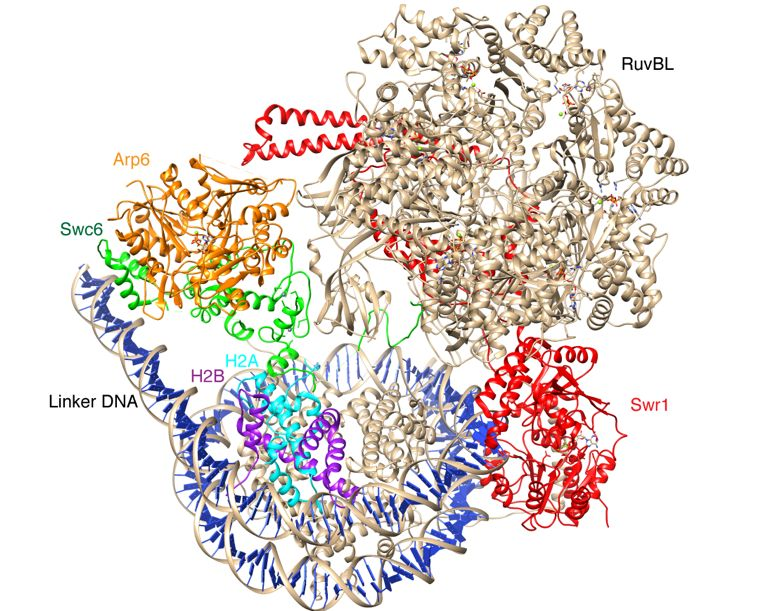
\includegraphics{SWR1_complex}
  \caption{酵母菌SWR1复合物}
  \label{fig:swr1_complex}
\end{figure}
生物实验中检测蛋白质复合物主要通过串联亲和纯化与质谱分析\cite{g_generic_1999}、酵母双杂交\cite{li_identification_1993}两种技术对蛋白质复合物进行分离和鉴定。串联亲和纯化与质谱分析通过靶蛋白标定以及自然条件下亲和纯化获取可能的蛋白质复合物,再使用质谱分析进行鉴定。酵母双杂交技术利用转录调控因子中的组件特征研究蛋白质之间的相互作用关系。虽然基于实验测定的方法具有生物学上的可解释性,但是生物实验往往条件困难、实验步骤多且成本昂贵,无法满足快速增长的研究需求。

蛋白质与生理环境存在广泛的相互作用,蛋白质复杂功能的实现同蛋白质之间、DNA与蛋白质、RNA与蛋白质的相互作用密切相关,蛋白质复合物正是一组强相关的蛋白质组合共同作用的结果。随着生物信息学的发展以及高通量技术的发展,蛋白质相互作用关系(Protein-ProteinInteraction,$PPI$,后简称为互作关系)得到了大量的补充,促成了大规模互作网络的构建\cite{butland_interaction_2005},即蛋白质相互作用网络(Protein-ProteinInteractionNetwork,$PIN$)。图\ref{fig:ppi}为酵母菌蛋白质相互作用网络。
\begin{figure}[htbp]
  \centering
  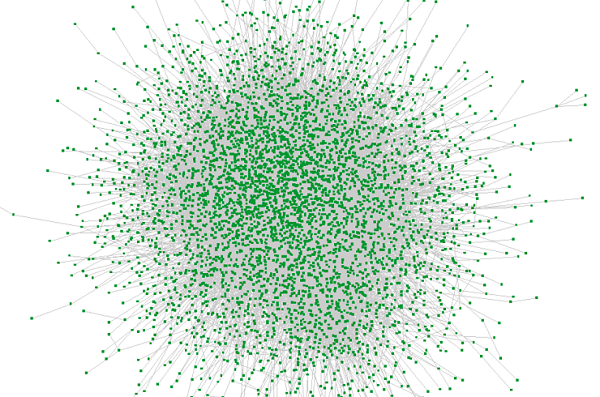
\includegraphics{ppi}
  \caption{酵母菌蛋白质相互作用网络}
  \label{fig:ppi}
\end{figure}
已知的蛋白质复合物可以视作互作网络里面的一系列子网络,因此利用图论和计算模型学习子网络的分布模式,即可在互作网络中发掘潜在的蛋白质复合物\cite{legrain_proteinprotein_2001}。利用图论的方法,蛋白质互作网络可以转换为无向图~$G=(V,E)$。其中$V$为图中结点的集合,表示所有的蛋白质,$E$为图中邻边的集合,表示所有的蛋白质互作关系。$PIN$转换为图结构之后,图论上的计算模型和深度学习方法就可以迁移到蛋白质复合物的研究中。2002年,Tong\cite{tong_combined_2002}等人提出了密集子图的假说,蛋白质复合物在$PIN$是密集链接的子图,而与其他的蛋白质连接相对稀疏。在$PIN$中预测蛋白质复合物的问题就转换为了密集子图的挖掘问题,逐渐发展出了利用$PIN$和计算方法识别蛋白质复合物的理论。

\section{国内外研究现状}
\label{section:research}

现有的基于计算方法的蛋白质复合物预测方法主要分为五类:基于网络结构的图聚类方法、融合生物信息的图聚类方法、核心附属扩展方法、动态网络方法以及监督学习方法。以下分别对这五类方法的研究现状做简单的介绍。

\subsection{基于网络结构的图聚类方法}
\label{section:TopologyMethod}

现有大多数复合物预测方法为基于网络结构的图聚类方法,基本思路是在无权无向图中挖掘密集子图。这类方法较为简单明确,取得了一定的成果。

MCODE算法\cite{bader_automated_2003}是最早提出基于网络结构构造密集子图的复合物预测算法。首先算法会计算所有结点的局部邻居密度,其中密度超过平均值的结点成为种子,视作初始子图。满足相应阈值条件的邻居结点不断扩充子图,直到阈值条件饱和,最终子图视为预测的复合物,算法最终会过滤掉结点数少的复合物。
Clique算法\cite{spirin_protein_2003}通过穷举法、超顺磁性聚类和蒙特卡洛模拟三种方法搜索完全图来检测蛋白质复合物。
RNSC算法\cite{king_protein_2004}以随机聚簇最为初始聚簇,按照代价函数逐渐削减聚簇,最终形成蛋白质复合物。
Pereira‐Leal\cite{pereiraleal_detection_2004}提出将马尔科夫聚类算法应用于蛋白质复合物检测,通过转移矩阵的自乘来扩展连通区域,通过幂运算进行膨胀操作只保留生成概率高的区域。膨胀和扩展操作交替运行,收敛之后获得蛋白质复合物。
LCMA算法\cite{li_interaction_2005}从蛋白质相互作用网络中较小的完全图开始,通过不断合并重合率高的完全图来检测蛋白质复合物。CFinder算法\cite{adamcsek_cfinder_2006}进一步定义了搜索与合并的策略,算法首先寻找网络中的k阶完全图,如果两个子图之间有k-1个公共结点,则定义为两个k阶完全图相邻,将两个子图合并。算法通过不断合并k阶完全图预测蛋白质复合物。
SCAN算法\cite{mete_structural_2008}认为一对蛋白质的公共邻居超过阈值时,这对蛋白质可被视为结构可达,可以作为种子蛋白质继续扩展其余结构可达蛋白质。
ClusterONE算法\cite{nepusz_detecting_2012}充分利用了蛋白质复合物内部连接密集,外部连接稀疏的假设,并且明确定义了子图紧密性。其主要思路是首先按照结点度排序获取种子结点,种子结点向外扩展操过程中可以添加或删除结点,以达到局部子图最佳紧密性。Zheng等人\cite{zheng_jiyu_2020}进一步改进了图紧密性定义,提出根据子图中3阶完全图个数来定义局部子图连紧密性。

有部分研究将$PIN$中的结点做预分类以达到更优的结果,CPridict和CODEC方法。

\subsection{网络预处理的图聚类方法}
\label{section:appendBiology}
蛋白质复合物的预测是一个复杂的生物学问题,而由于实验手段的限制,蛋白质相互作用网络的数据存在着高假阴性和高假阳性的缺陷\cite{von_mering_comparative_2002}。研究者开始尝试融合生物数据,对网络拓扑结构进行修复和加权处理,提高$PIN$的可信度以获取更精确的聚类结果。
DPClus算法\cite{altaf-ul-amin_development_2006}最早对$PIN$做加权处理,根据一对结点公共邻居数量给这对结点之间的边加权,结点的权重所有邻边的权重之和。权重较大的结点作为种子结点,通过紧密型结点的连接预测蛋白质复合物。
PCP算法\cite{chua_using_2008}利用使用FS-weight计算网络的权重

\subsection{核心附属扩展方法}
\label{section:CoreAppend}
SCAN算法\cite{mete_structural_2008}已经提出了扩展的思想。然而这只是拓扑结构上的核心思想,真正的核心思想是核心蛋白质,生物学上发现这类蛋白质有什么属性。。。对复合物有什么影响,如图\ref{fig:core_append}所示

\begin{figure}[htbp]
  \centering
  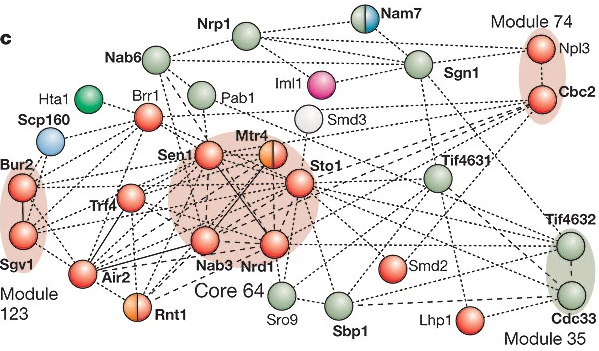
\includegraphics{core_append}
  \caption{核心附属结构示例——Core64部分为核心结构}
  \label{fig:core_append}
\end{figure}

ClusterONE算法\cite{nepusz_detecting_2012}
\subsection{监督学习方法}
\label{section:Supervision}
包括监督下的方法
\subsection{动态网络方法}
\label{section:Dynamic}


\subsection{方法总结}
\label{section:researchSummary}

\section{研究动机和思路}
\label{section:motivation}

国内外学者对复合物的识别已经提出了诸多方法,总体趋势也是趋向于融合生物数据和网络数据并达到更精确的预测,但是目前现有的方法还存在以下的不足。
\begin{itemize}
  \item 无法利用已有的先验知识。上述的研究方法主要是基于无监督方法,在复合物的研究问题上,无监督方法具有训练简单、结构明确的优点。再如今实验技术更新、生物数据量增加以及图数据挖掘算法井喷发展的情况下,无监督学习方法无法利用已有的先验知识。
  \item 复合物准确度较低。部分模型方法如RNSC算法\cite{king_protein_2004}、Clique算法\cite{spirin_protein_2003}等等具有很强的随机性,倾向于这类方法为了达到较高的复合物召回率,往往倾向于产生过量的候选复合物,导致结果的准确率的降低,大量非复合物预测成立复合物,这样的数据对以后的使用不好。
  \item 生物信息在$PIN$中融合度低。在\ref{section:appendBiology}中提到了融合生物信息的诸多方法,然而这些方法只停留在利用生物信息更改$PIN$邻边权重的层面,不同的生物信息如GO注释、基因表达信息、蛋白质保守性等数据被统一编码到了相互作用的边权重中,这个编码转换过程会丢失原有丰富的生物数据。编码过程仅仅作为$PIN$数据的预处理,生物数据无法动态地参与到复合物预测模型的框架设计中。同时,目前也没有方法将生物信息编码到蛋白质结点中,如何有效的利用结点编码增强复合物的预测质量也是一个亟待解决的问题。
\end{itemize}

针对以上的问题。
研究动机:RNSC算法\cite{king_protein_2004}削减的思想,Clique算法\cite{spirin_protein_2003}过多样本,Pereira‐Leal\cite{pereiraleal_detection_2004}融合了总体拓扑结构
\section{研究工作和成果}
\label{section:workandresult}

\section{论文组织}
\label{section:organization}
\chapter{数据处理}
\label{chapter:dataprocess}

\section{特征工程}
\label{section:featEngineer}
\subsection{蛋白质功能注释特征}
\label{subsection:GoSimilarity}

基因本体信息\cite{ashburner_gene_2000}即GO注释信息是描述蛋白质功能表达的词汇表,将生物活动过程进行统一编码表示,其在生物信息学邻域得到了广泛的应用。对应到蛋白质中,蛋白质分子参与的若干生物过程均可对应到GO注释表,形成对该蛋白质的综合功能描述。GO注释项总体分为三类,分别是生物过程(Biological Process)、分子功能(Molecular Function)及细胞组成(Cellular Component),生物过程描述分子功能有序组成的生命活动,分子功能描述分子在生物学上的活性,细胞组成描述了亚细胞结构及位置信息。GO注释项之间由于描述涵盖范围的不同,具有一定的从属关系,所有的GO注释项可以组成有向无环图(Directed Acyclic Graph,简称DAG)。图\ref{fig:go-dag}为QuickGO\cite{binns_quickgo_2009}网站中获取的生殖细胞发育过程对应的GO注释DAG图。GO注释信息的从属关系主要分为两种,分别是$is\_a$和$part\_of$,其中$is\_a$表示包含关系,如图中黑色箭头所示,$part\_of$表示从属关系,如图中蓝色箭头所示。图中每一个方框展示了GO注释项及其生物功能。
\begin{figure}[htbp]
    \centering
    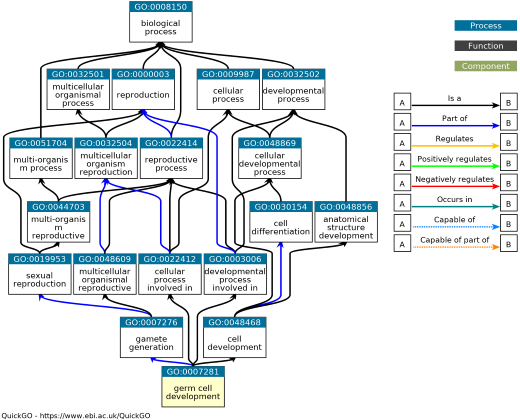
\includegraphics{go-dag}
    \caption{生殖细胞发育对应的GO示意图}
    \label{fig:go-dag}
\end{figure}

通常情况下,蛋白质复合物中蛋白质倾向于相同的功能表达,同时功能表达相似性越高时,蛋白质产生相互作用的可能性越大。部分算法\cite{ulitsky_identification_2007,jianxing_feng_max-flow-based_2011}基于功能表达数据提出了$PIN$连边权重更新的方法。
本文采用两种方法计算蛋白质功能相似度,将计算结果作为$PIN$网络中邻边的蛋白质功能特征。

第一种蛋白质功能相似度计算方法为Wang等人\cite{wang_new_2007}提出的方法。

给定一个GO注释项$p$,从GO的总体DAG图中提取子图$DAG_p(A,T_p,E_p)$,其中$T_p$是$p$及所有$p$的祖先结点的注释项,$E_p$表示所有截取的注释项的连接关系。
定义$T_p$中每一个结点对$p$的语义值如下:
\begin{equation}
    \label{equ:feat:go:SAT}
    S_p(t)=\left\{\begin{array}{l}
        1,t=p                                                                        \\
        \max {\{ w_e\times S_p(t^\prime )| t^\prime\in ~children~of~(t) \} },t\neq p \\
    \end{array}\right.
\end{equation}
其中$w_e$是$t^\prime$和$t$之间的权重,定义两种类型的边$is\_a$和$part\_of$权重各自为0.8和0.6。有公式可以直观得出,祖先结点点中离$p$注释越远的注释项,其对$p$的语义值越小,而$p$对自身的语义值贡献为1。
定义了所有祖先结点对$p$的语义值之后,可以直接得出$p$的语义值得分,计算公式如下:
\begin{equation}
    \label{equ:feat:go:SVA}
    SV(p)=\sum_{t \in T_p}(t)
\end{equation}
按照该计算方法,可以得到每一个注释项各自的语义值,在此基础上可以得到两个注释项$p$,$q$语义值的相似度,具体计算方法如下:
\begin{equation}
    \label{equ:feat:go:SimItemWang}
    Sim_{GO}(p,q)=\frac{\sum_{t \in T_p \cap T_q}(S_p(t)+S_q(t))}{SV(p)+SV(q)}
\end{equation}
其中$t$为$p$和$q$的所有公共祖先结点。由于蛋白质通常是由多个注释项组成,因此蛋白质之间的功能相似性需要考虑两个蛋白质各自注释项之间的综合结果,其具体计算方法如下:
\begin{equation}
    \label{equ:feat:go:SimProteinWang}
    \begin{aligned}
        Sim_{Protein}(P,Q) & =\frac{1}{m+n}\cdot \left\{\sum_{1\leq i\leq m}{\max_{1\leq j\leq n}[{Sim_{GO}(p_i,q_j)}}]\right. \\
                           & \left.+\sum_{1\leq j\leq n}{\max_{1\leq i\leq m}[{Sim_{GO}(p_i,q_j)}}]\right\}
    \end{aligned}
\end{equation}
其中$P$,$Q$表示两个蛋白质,其中分别具有$\{p_i| i=1,2,\dots,m\}$,$\{q_j| j=1,2,\dots,n\}$的功能注释项。
这个方法的核心思想是将两个蛋白质的注释信息相互关系矩阵$m\times n$构造出来,只考虑源蛋白质的某一个注释项和目标蛋白质所有注释项最大的相关性,而蛋白质的相互作用关系是所有最大值的平均。

第二种蛋白质功能相似度计算方法为Lin等人\cite{lin_information-theoretic_1998}提出的方法。首先计算某两个注释项之间的相关性,具体计算过程如下:
\begin{equation}
    \label{equ:feat:go:SimItemLin}
    Sim_{GO}(p,q)=\min_{anc \in Ancient(p,q)}\mathcal{P} (anc)
    % Sim_{GO}(p,q)=\max{\frac{2\times \log }{} }
\end{equation}
其中$Ancient(p,q)$表示两个注释项的公共祖先,而$\mathcal{P}$表示某一个注释项在所有蛋白质中出现的概率。这个计算公式直观的认为,两个具有相互关联的功能注释,其关联结点越稀有,则表示两个注释项的相关性越强。计算蛋白质功能相似性的计算方法如下:
\begin{equation}
    \label{equ:feat:go:SimProteinLin}
    Sim_{Protein}(P,Q)=\max{\frac{2\times \log \{Sim_{GO}(p,q)\}}{\log {\mathcal{P}_p}+\log {\mathcal{P}_q}} }
\end{equation}


\subsection{蛋白质结构域特征}
\label{subsection:domainSimilarity}
蛋白质结构域时蛋白质具有独立功能和特异结构的区域,结构域互作信息影响蛋白质复合物的形成\cite{kim_relating_2006}。结构域之间具有相互作用关系,这些相互作用关系可以从三维交互域(3did)数据库\cite{mosca_3did_2014}提取,并构建成结构域相互作用网络(Domain-Domain Interaction Network,简称DDI)。
单个蛋白质所具有的结构域可以映射到结构域互作网络的若干结点,成为一个结构域集群,而蛋白质域相似性可以转换为两个结构域集群的相互作用关系。
本文中两个蛋白质的结构域互作特征包括如下方面:两个蛋白质结构域交集、并集以及相互之间的差集;映射到结构域相互网络之后,两个结构域集群之间的相互作用关系数量,其具体的计算公式如下。
\begin{equation}
    \label{equ:feat:domain}
    Sim_{domain} = \sum_{i \in dom(p)}{\sum_{j \in dom(q)}{Weight_{ij}}}
\end{equation}
其中$i$、$j$分别时蛋白质$p$、$q$之间的结构域,$Weight_{ij}$代表结构域$i$、$j$在结构域相互作用网络中的作用强度,对于无权网络可以取值为1。

huang等人\cite{huang_protein-protein_2013}在运用结构域相互作用网络预测蛋白质相互作用时,提出了使用一阶邻居和二阶邻居计算$domain$相似性的想法,其扩展方式如图\ref{fig:domain-second}所示。本文也同时补充了一阶和二阶扩展之后的蛋白质$domain$相似性特征。
\begin{figure}[htbp]
    \centering
    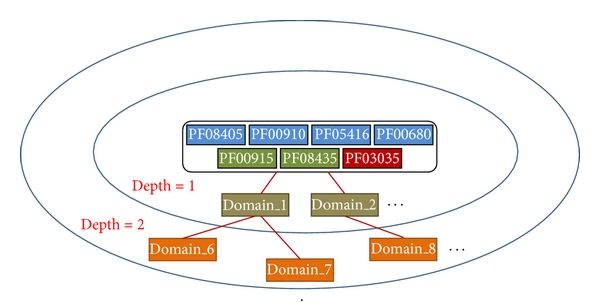
\includegraphics{domain-second}
    \caption{DDI多阶邻居示意图}
    \label{fig:domain-second}
\end{figure}


\subsection{蛋白质亚细胞特征}
\label{subsection:SubcellSimilarity}
细胞是一个高度有序的结构,胞内根据空间分布和功能不同,可以分成不同细胞器或细胞区域,蛋白质只有转运到正确的部位才能参与细胞的各种生命活动,ZHANG等人\cite{zhang_protein_2007}认为蛋白质的亚细胞定位有助于研究蛋白质的生物学功能,同时对蛋白质的其他研究如相互作用、进化等也能提供必要的信息。huang等人提出\cite{huang_genome-wide_2017}使用蛋白质复合物和亚细胞定位信息预测关键蛋白质,蛋白质复合物,蛋白质复合物的生成和功能实现和其所处的细胞位置相关,因此蛋白质的亚细胞定位能对蛋白质复合物的形成产生一定的影响。本文将两个蛋白质亚细胞定位数据的交集和并集作为蛋白质的亚细胞定位特征。图\ref{fig:subcell}为苏氨酸蛋白激酶TOR1亚细胞定位图,其中黄色的部分表示其主要的注释区域,包括细胞膜和液膜。

\begin{figure}[htbp]
    \centering
    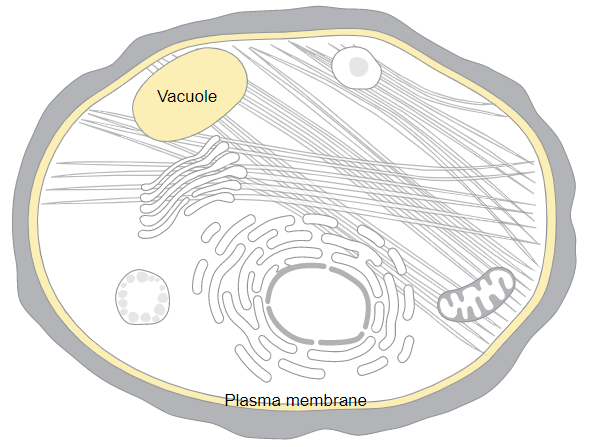
\includegraphics{subcell}
    \caption{苏氨酸蛋白激酶TOR1亚细胞定位图}
    \label{fig:subcell}
\end{figure}

\subsection{蛋白质拓扑特征}
\label{subsection:TopoSimilarity}


\section{PIN及数据集构建}
\label{section:datasetsConstruct}
\subsection{网络结构构建}
\label{subsection:NetConstruc}
\subsection{数据集提取与划分}
\label{subsection:datasetExtract}
\subsection{子图特征}
\label{subsection:subgraphFeat}

\section{相关评价指标}
\label{section:metrix}
\chapter{复合物筛选模型设计}
\label{chapter:gcnfilter}

\section{相关算法介绍}
\label{section:arithmetic}
\subsection{网络嵌入}
\label{subsection:nodeEmbedding}
\subsection{图卷积神经网络}
\label{subsection:GCN}
\subsection{图自编码器}
\label{subsection:GAE}
\section{算法总体流程}
\label{section:progress}
\section{基于生物特征的模型}
\label{section:biofeatBaseModel}
可添加的特征包括蛋白质功能注释特征、结构域特征、亚细胞定位特征以及网络拓扑特征。参照\ref{section:featEngineer}介绍的特征提取方法,$PIN$中每条相互作用边所具有的特征维度为{},具体分布如表\ref{tab:PINedgeFeatNUms}所示:
\begin{table}[h]
    \centering
    \caption{$PIN$边特征维度分布}
    \label{tab:PINedgeFeatNUms}
    \begin{tabular}{C{3cm}C{3cm}C{3cm}C{3cm}}
        \toprule
        \textbf{功能注释特征} & \textbf{结构域特征} & \textbf{亚细胞定位特征} & \textbf{网络拓扑特征} \\
        \midrule
        2                     & 7                   & 2                       & 2                     \\
        \bottomrule
    \end{tabular}
\end{table}
生物上的,拓扑上的,异常数据处理,过大数据归一化
\section{基于全局特征的模型}
\label{section:GlobalfeatBaseModel}
GAE怎么做的,deepwalk怎么做的,node2vec怎么做的
\section{特征融合模型}
\label{section:fusionfeatBaseModel}
考虑少量蛋白质特征,考虑图拓扑特征
\section{尺寸敏感性的图读出算法}
\label{section:GPool}

\chapter{实验结果与分析}
\label{chapter:resultAndOther}
\chapter{具有尺寸敏感性的复合物筛选模型}
\label{chapter:poolfilter}
\chapter{总结与展望}
\label{chapter:SummaryAndForward}
% 参考文献
\printTJbibliography
\end{document}
